\documentclass[10pt, a4paper, oneside]{ctexbook}
\usepackage{amsmath, amsthm, amssymb, bm, graphicx, mathrsfs,esint,wrapfig,color,xcolor}
\usepackage{hyperref}
\hypersetup{hypertex=true,
            colorlinks=true,
            linkcolor=blue,
            anchorcolor=blue,
            citecolor=blue}%用于公式引用
\title{{\Huge{\textbf{数学物理方法}}}\\Mathematical Methods in Physics}
\author{YLJ a.k.a. Natyiano}
\date{\today}
\linespread{1.5}
\newtheorem{theorem}{定理}[section]
\newtheorem{definition}[theorem]{定义}
\newtheorem{lemma}[theorem]{引理}
\newtheorem{corollary}[theorem]{推论}
\newtheorem{example}[theorem]{例}
\newtheorem{proposition}[theorem]{命题}
\newtheorem{method}[theorem]{方法}
\def\D{\mathrm{d}}
%\def\F{\ensuremath{f(z)}}
\def\Fex{\ensuremath{u(x,y)+iv(x,y)}}
\def\de{\ensuremath{\Delta}}
\newcommand{\partdev}[3][]
{\ensuremath{\frac{\displaystyle \partial^{#1} #2}{ \displaystyle \partial #3}}}
\newcommand{\F}[1][z]
{\ensuremath{f(#1)}}
\newcommand{\dev}[3][]
{\ensuremath{\frac{\displaystyle \D^{#1} #2}{ \displaystyle \D #3}}}
\begin{document}


\maketitle

\pagenumbering{roman}
\setcounter{page}{1}
\newpage
\pagenumbering{Roman}
\setcounter{page}{1}
\tableofcontents
\newpage
\setcounter{page}{1}
\pagenumbering{arabic}

\chapter*{复变函数部分}
\chapter{复数}
\textbf{约定}:
我们认为$z\in \mathbb{C}$,$x,y \in \mathbb{R}$
\section{定义以及运算}

\begin{definition}
    $$i=\sqrt{-1}$$
\end{definition}
称之为虚数单位。通过虚数单位和『实数单位($1$)』的线性组合,可以得到任意复数的表示方式:
$$z=x+iy,\;z\in \mathbb{C}, x\&y \in \mathbb{R}$$
$x,y$分别称为实部和虚部,记为:
\begin{align*}
    x=\text{Re}\;z\\y=\text{Im}\;z
\end{align*}
\begin{definition}
    $$z^*=x-yi$$
\end{definition}
称为$z$的共轭复数。容易得到,
\begin{align*}
    &z\cdot z^*=x^2+y^2=|z|^2 \ge 0 \\
    &x=\text{Re}\;z=\frac{z+z^*}{2} \\
    &y=\text{Im}\;z=\frac{z-z^*}{2i}
\end{align*}
注意到复数的运算与实数的运算存在许许多多的不同之处,例如
\begin{example}
    $$\lim_{y\to0}\frac{1}{x+yi}\ne \frac{1}{x}$$
    \begin{align*}
    \lim_{y\to0}\frac{1}{x+yi}=\lim_{y\to0}\frac{x-yi}{x^2+y^2}\to\\ \text{\rm Re} \;z= \begin{cases}
        0,\;x=0\\\displaystyle \frac{1}{x},\; x\ne 0
    \end{cases}\text{\rm Im} \;z= -i\pi \delta(x)
    \end{align*}
\end{example}
\section{复数的几何表示}
引入复平面可以容易地表示复数的几何形式:即$z=x+yi$在$x$轴(实轴)上的投影为$x$,在$y$轴(虚轴)上的投影为$y$。
那么,对应向量的(主)辐角$\theta$ 以及模$\rho$便定义为:
\begin{definition}
    $$\theta=\text{\rm Arg } z;\;\;\rho=\sqrt{x^2+y^2}$$
\end{definition}
主辐角记为Arg $\displaystyle z \in[-\pi,\pi] =\arctan \frac{y}{x}$,辐角记为arg $z$
那么得到:
\begin{lemma}
    \label{eularq}
    $$
    z = \rho(\cos \theta + i \sin \theta)
    $$
\end{lemma}
注意到:
$$
\frac{1}{z}=\frac{1}{\rho(\cos \theta + i \sin \theta)}=\frac{1}{\rho}(\cos \theta - i \sin \theta)
$$
\begin{lemma}
    \label{le1}
    假设$1/z=n\in \mathbb{C}$,
    $$\rho_{n}=1/\rho_z;\;\; {\rm arg \;} z=-{\rm arg \;} n$$
\end{lemma}
同样
\begin{lemma}
    \label{le2}
    假设$$
    z=\prod_{i=1}^{n}z_i\to \rho_z=\prod_{i=1}^n \rho_{z_i};\quad \text{\rm arg }z=\sum_{i=1}^n \text{\rm arg }z_i
    $$
    $$z_i\in\mathbb{C}$$
\end{lemma}
\begin{theorem}
    de Moivre’s 定理:
    $$z_1=\rho_1(\cos\theta_1+i\sin \theta_1)\quad z_2=\rho_2(\cos\theta_2+i\sin \theta_2)$$
    $$\Rightarrow$$
    $$z_1\cdot z_2=\rho_1\rho_2(\cos(\theta_1+\theta_2)+i\sin(\theta_1+\theta_2))$$
\end{theorem}
结合\ref{le1}和\ref{le2},我们可以得到任意个复数的乘法除法公式:
\begin{corollary}
    \begin{align*}
        z=\frac{\displaystyle\prod_{i=1}^n a_i \in \mathbb{C} }{\displaystyle\prod_{i=1}^n b_i \in \mathbb{C}}
        :\Longrightarrow \rho_z=\frac{\displaystyle\prod_{i=1}^n \rho_{a_i}}{\displaystyle\prod_{i=1}^n \rho_{b_i}} \quad \text{\rm arg }z = 
        \sum_{i=1}^n \text{\rm arg }a_i - \sum_{i=1}^n \text{\rm arg }b_i
    \end{align*}
\end{corollary}
\section{复数数列}
形式如下的序列称为复数数列
$$
z_n=x_n+i y_n , \; \; n=1,2,3,4,\dots
$$
$$z_n\text{ 收敛} \Leftrightarrow x_{n},y_{n} \text{ 收敛} $$
\section{欧拉公式以及复数的指数函数形式}

\begin{theorem}
    欧拉公式:
    $$e^{i\theta}=\cos \theta + i \sin \theta$$
\end{theorem}
\begin{proof}
    由 Taylor-Sereis
$$
e^x= \sum_{n=0}^\infty \frac{x^n}{n!}
$$
得到
$$
e^{i\theta}= \sum_{n=0}^\infty \frac{i^n\theta^n}{n!}=\left[ 1-\frac{\theta^2}{2}+\frac{\theta^4}{4!}+\dots \right]+ i \left[ \theta-\frac{\theta^3}{3!}+\dots \right]
$$
考虑到$\cos \theta$和$\sin \theta$ 的 Taylor-Series,得到:
$$
e^{i\theta}= \cos \theta + i \sin \theta
$$
\end{proof}
显然如上的证明并不是一个严格的证明,因为我们没有证明如上的展开适用于复数域,以及在交换次序时没有事先证明它绝对收敛。
结合\ref{eularq}得到$$z=\rho e^{i\theta}$$称为复数的指数函数形式。
\begin{example}
    计算无穷级数:$\cos \theta + \cos 2\theta + \cos 3\theta + \dots$
\end{example}
\begin{proof}
    原式等价于
    \begin{align*}
        \mathrm{Re} \;\; [e^{i\theta}+e^{i2\theta}+e^{i3\theta}+\dots]
    \end{align*}
    \begin{align*}
        e^{i\theta}+e^{i2\theta}+e^{i3\theta}+\dots\\
        =\lim_{n\to \infty} \frac{\displaystyle e^{i\theta}-e^{i(n+1)\theta}}{\displaystyle 1-e^{i\theta}}
    \end{align*}
\end{proof}

\section{复数域上的指数函数的反函数}
对于$\forall \; z\in \mathbb{C}$, 如何定义函数$g=f(z)=e^{z}$ 的反函数?
即定义一个函数,使得:
\begin{equation*}
    f^{-1}(g)=z
\end{equation*}
这个函数称为复对数函数,区别于$\mathbb{R}$上的指数函数$\ln(x)$。
\begin{definition}
    复对数函数:$$\mathrm{Ln}\;z=\ln |z| + i\mathrm{arg} \;z +2n\pi i$$
    $$s.t. \mathrm{Ln}\;g  = \mathrm{Ln}\; |z|e^{i\mathrm{arg}\;z+2ni\pi} $$
\end{definition}
其多值性来源于
$$
g=e^z=e^{z+2ni\pi}
$$

\chapter{复变序列}
对于某一复数序列$u_n=x_n+iy_n$,其和前$n$项和$S_n$:
\begin{equation*}
    \begin{aligned}
    &\sum_{n=0}^{\infty}\left(x_{n}+i y_{n}\right) \\
    &S_{n}=X_{n}+i Y_{n} \\
    &X_{n}=\sum_{i=0}^{n} x_{i}, Y_{n}=\sum_{j=0}^{n} y_{j}
    \end{aligned}
\end{equation*}
无穷级数收敛的充要条件:
$\forall\; \varepsilon > 0,\;\; \exists\; n>0;\;\; n \in \mathbb{Z}, \; s.t.\;\; \forall \; p>0\:$
\begin{equation*}
    \left|u_{n+1}+u_{n+2}+\ldots+u_{n+p}\right|<\varepsilon
\end{equation*}
级数收敛的必要条件:
\begin{equation*}
    \text{\boldmath Preliminary Test: } \lim_{n\to \infty} u_n = 0
\end{equation*}
\section{级数收敛性判别法}
\textbf{Test for alternating series}: An alternating series converges if the absolute value of the terms decreases steadily to zero, that is, if $\color{red} \left|a_{n+1}\right| \leq\left|a_{n}\right|$ and $\color{blue} \lim _{n \rightarrow \infty} a_{n}=0$.
\textbf{\color{red} 一致递减 \color{blue}至0}

\textbf{Comparison Method: }If $\exists N \in \mathbb{N}, \forall n>N$, the condition $\left|u_{n}\right|<v_{n}$ is satisfied. If $\displaystyle \sum_{n=0}^{\infty} v_{n}$ are convergent, then $\displaystyle \sum_{n=0}^{\infty}\left|u_{n}\right|$ are convergent.

\textbf{Ratio Method: }If there exists a constant $\rho$ ({\color{red} un-correlated with $n$ }), and $\left|u_{n+1} / u_{n}\right|<\rho<1$, then $\displaystyle \sum_{n=0}^{\infty} u_{n}$ are absolutely convergent.

\textbf{d'Alembert Method(Criterion): }级数的通项比值$\left(\displaystyle \frac{u_{n+1}}{u_n}\right)$的{\color{red}模}的上极限小于$1$,则原级数绝对收敛;级数的通项比值的模下极限大于1,则原级数发散。

\textbf{Gauss Method: }Assume that the ratio between two neighboring terms has the following form: $\displaystyle \frac{u_{n}}{u_{n+1}}=1+\frac{\mu}{n}+O\left(n^{-\lambda}\right)$
where $\mu=a+i b, \lambda>1$. 

If $a>1$, $\displaystyle \sum_{n=0}^{\infty} u_{n}$ absolutely convergent. 

If $\displaystyle a \leq 1, \sum_{n=0}^{\infty}\left|u_{n}\right|$ divergent.

\begin{example}
    使用 {\rm Gauss Method} 判别 级数$\displaystyle S_n=\sum_{n=0}^\infty \frac{1}{n}$的收敛性:
    \begin{align*}
        \frac{u_n}{u_{n+1}}=\frac{n+1}{n}=1+\frac{1}{n}
    \end{align*}
    则$a=1$,原级数发散。
    \newline
    使用 {\rm Gauss Method} 判别 级数$\displaystyle S_n=\sum_{n=0}^\infty \frac{1}{n^2}$的收敛性:
    \begin{align*}
        \frac{u_n}{u_{n+1}}=\left(\frac{n+1}{n}\right)^2=1+\frac{1}{n^2}+\frac{2}{n}
    \end{align*}
    则$a=2$,原级数绝对收敛。
\end{example}

\textbf{Cauchy Method: }$\displaystyle |u_n|^{1/n}$的上极限小于$1$,原级数绝对收敛;大于$1$,原级数发散。

\section{复数序列的一致收敛}

如果$S_n$一致收敛,则:
\begin{itemize}
    \item Continuity $u_{k}(z)$ is continuous in $G$, and $\sum_{k=1}^{\infty} u_{k}(z)$ is uniformly convergent, then $S(z)=\sum_{k=1}^{\infty} u_{k}(z)$ is continuous in $G$
    \item $\displaystyle
    \int_{C} \sum_{k=1}^{\infty} u_{k}(z) \D z=\sum_{k=1}^{\infty} \int_{C} u_{k}(z) \D z
    $
    \item $\displaystyle
        f(z)=\sum_{k=1}^{\infty} u_{k}(z) \text { is analytic in } G \to
        f^{(p)}(z)=\sum_{k=1}^{\infty} u_{k}^{(p)}(z)
        $
\end{itemize}

\section{幂级数与阿贝尔定理}

对于幂级数
\begin{equation*}
    \sum_{n=0}^{\infty} c_{n}(z-a)^{n}=c_{0}+c_{1}(z-a)+c_{2}(z-a)^{2}+\ldots
\end{equation*} 有
\begin{theorem}\rm
    \textbf{Abel theorem}: If the series $\displaystyle \sum_{n=0}^{\infty} c_{n}(z-a)^{n}$ are convergent at $z=z_{0}$, then
the series are absolutely convergent in a disk region (with a radius of $\left|z_{0}-a\right|$ ) surrounding $z_{0}$, and are uniformly convergent in the region $|z-a| \leq r\left(r<\left|z_{0}-a\right|\right)$.
\end{theorem}
\begin{corollary}\rm
    If $\displaystyle \sum_{n=0}^{\infty} c_{n}(z-a)^{n}$ are divergent at $z_{1}$, then also divergent in $|z-a|>\left|z_{1}-a\right|$.
\end{corollary}

\begin{figure}[h]
    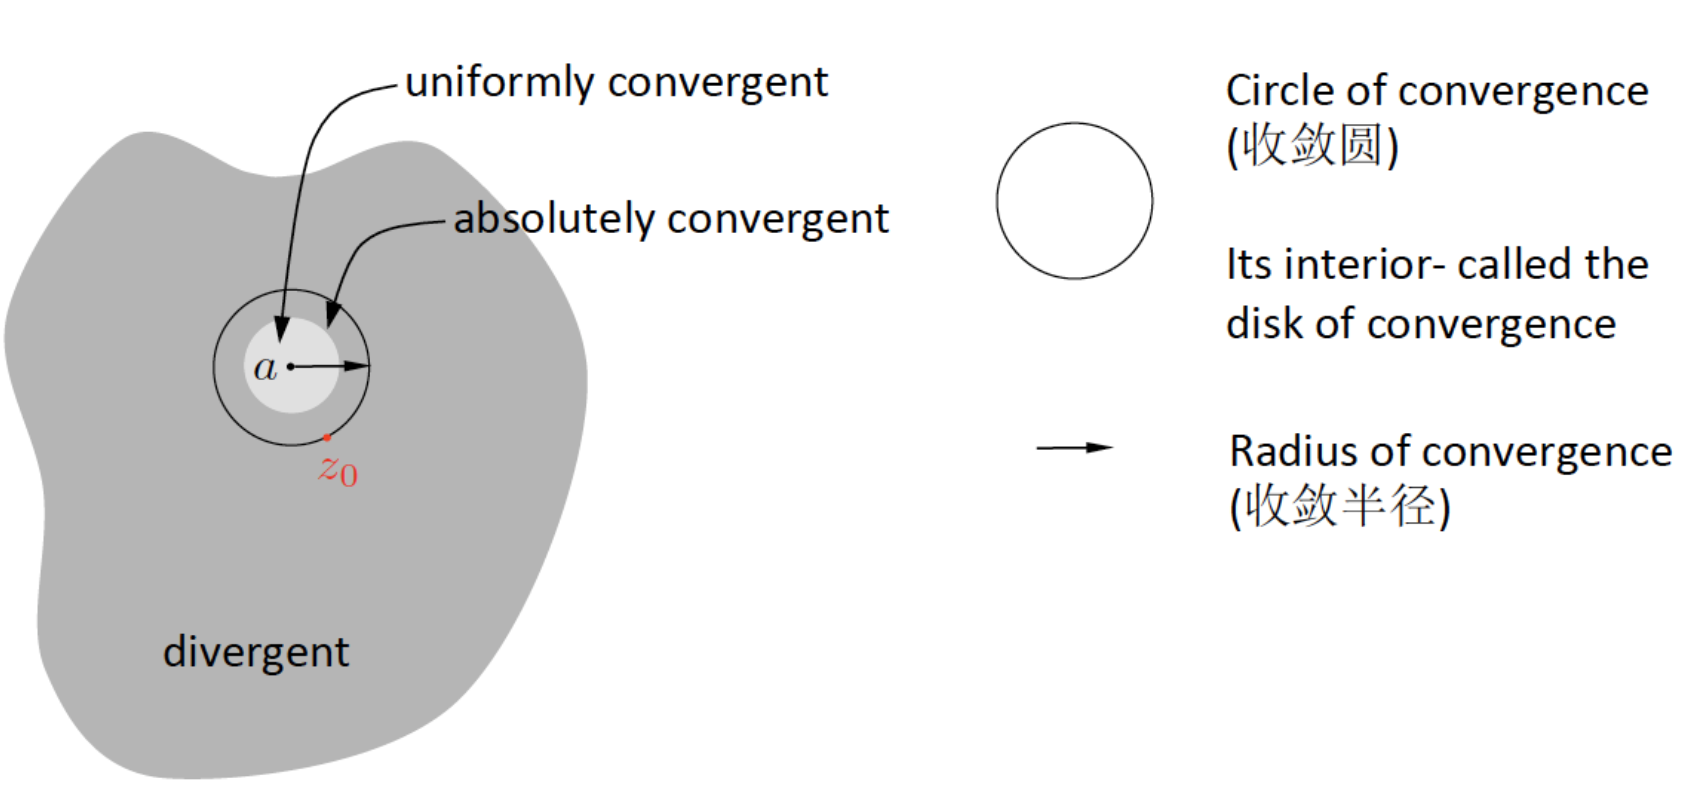
\includegraphics[width=0.9\textwidth]{./assets/converge_radius.png}
\end{figure}
计算幂级数的收敛半径的方法:
\begin{method}
    {\rm \textbf{Cauchy-Hadamard Formula: }}
    \begin{equation*}
        R=\frac{1}{\overline{\lim }_{n \rightarrow \infty}\left|c_{n}\right|^{1 / n}}=\underline{\lim }_{n \rightarrow \infty}\left|\frac{1}{c_{n}}\right|^{1 / n}
    \end{equation*}
\end{method}
\begin{method}
    {\rm \textbf{d'Alembert Critrion: }}
    \begin{equation*}
        R=\lim _{n \rightarrow \infty}\left|\frac{c_{n}}{c_{n+1}}\right|
    \end{equation*}
\end{method}

\chapter{复变函数}
\section{复变函数的概念}
\begin{definition}
    复变函数是复数区域到复数区域的映射。
    $$f:\mathbb{C}\to \mathbb{C}$$
    $$f(z)=u(x,y)+iv(x,y)\quad z=x+iy\quad x,y\in \mathbb{R}$$
\end{definition}
与实变函数不同,{\color{red}区域}与{\color{red}区间}是有显著差异的。
\begin{definition}
    如果复平面上的点集$D$ 满足以下条件:
    \begin{enumerate}
        \item 开集性:不包含边界。 $\forall \; z_0 \in D ,\quad \exists \; \epsilon >0 \quad s.t. \; \left\{ z\;\mid\;|z-z_0|<\epsilon \right\} \subset D $
        \item 连通性:任意两点之间可以用区域内的线连通。
    \end{enumerate}
    那么点集$D$称为(开)区域。
    闭区域$$\overline{D}=D+\partial D$$
    $\partial D$是$D$区域的边界。边界具有方向,其正方向定义为使得区域位于运动方向的左手侧的方向。
\end{definition}
\begin{definition}
    双曲函数定义为:
$$
\begin{array}{lll}
\sinh (z)=\displaystyle\frac{e^{z}-e^{-z}}{2} & \cosh (z)=\displaystyle\frac{e^{z}+e^{-z}}{2} & \tanh (z)=\displaystyle\frac{\sinh (z)}{\cosh (z)} \\
\operatorname{coth}(z)=\displaystyle \frac{\cosh (z)}{\sinh (z)} & \operatorname{sech}(z)=\displaystyle \frac{1}{\cosh (z)} & \operatorname{csch}(z)=\displaystyle \frac{1}{\sinh (z)}
\end{array}
$$
\end{definition}
类比$\cos z, \sin z$可以得到:
双曲函数的周期性:
$$
\sinh (z) = \sinh (z+i2n\pi) \quad \cosh (z) = \cosh (z+i2n\pi) \quad \tanh(z)=\tanh(z+in\pi)\quad n\in\mathbb{Z}
$$
\begin{definition}
    函数$f^{-1}(z)$称为函数$f(z)$的逆函数,如果:
    $$
    f^{-1}(f(z))=z
    $$
\end{definition}

\section{单值性与黎曼面}
注意函数的多值性:
\begin{figure}[h]
    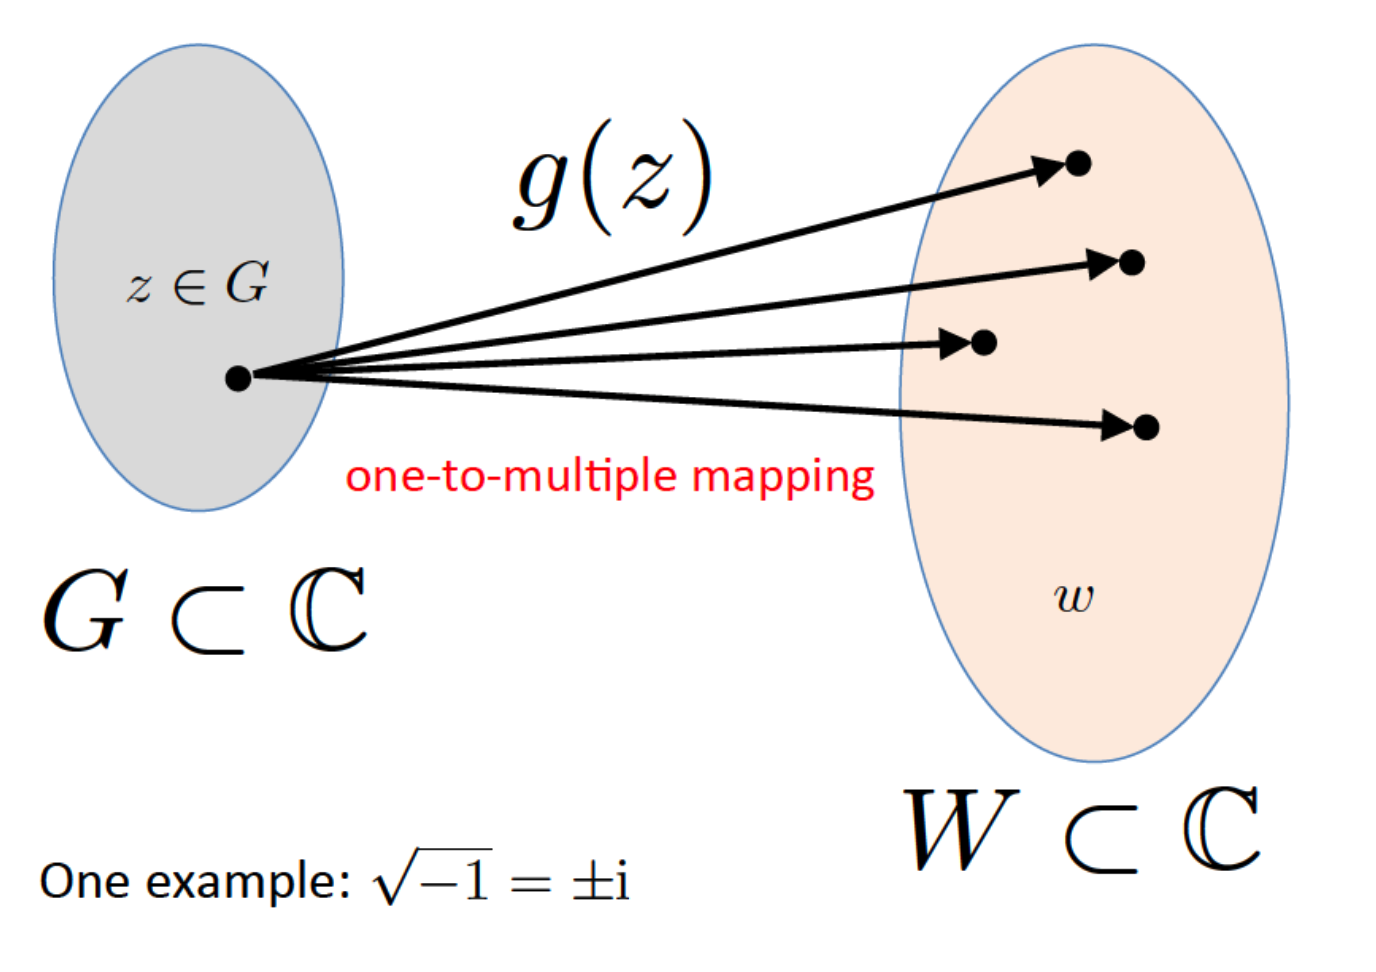
\includegraphics[width=0.9\textwidth]{./assets/multi-value.png}
\end{figure}
\begin{equation*}
    \text{定义域$G$}\quad z=x+i y \quad \xrightarrow{f(z)} \quad \text{值域$W$} \quad w=f(z)=u(x, y)+i v(x, y)
\end{equation*}
\begin{example}
    根式函数:$w=\sqrt[n]{z-a}$。令$z-a=re^{i\theta}$
    得到$w$有$n$个根:
    $$
    w_1=\sqrt[n]{r}e^{\theta/n}\quad
    w_2=\sqrt[n]{r}e^{\theta/n+2\pi/n}\quad
    \dots \quad
    w_n=\sqrt[n]{r}e^{\theta/n+2(n-1)\pi/n}
    $$
    辐角的多值性                                                           
\end{example}
\begin{example}
    对数函数:
$$
w=\ln z=\ln |z| +\textcolor{red}{i(\theta \pm 2n\pi)}
$$
\textcolor{red}{模的多值性}
\end{example}
反三角函数:
\begin{align*}
&\arcsin (z)=\frac{1}{i} \ln \left(i z+\sqrt{1-z^{2}}\right) \\ 
&\arccos (z)=\frac{1}{i} \ln \left(z+\sqrt{z^{2}-1}\right)\\ 
&\arctan (z)=\frac{1}{2 i} \ln \frac{1+i z}{1-i z}
\end{align*}
\begin{example}
    以$\arcsin z$为例:
    $$
\sin (w)=\frac{e^{i w}-e^{-i w}}{2 i}=z
$$
{\rm Multiply $e^{i w}$ for both sides, we have}
$$
\begin{aligned}
&\left(e^{i w}\right)^{2}-2 i z\left(e^{i w}\right)-1=0 \\
&e^{i w}=\frac{2 i z \pm \sqrt{4-4 z^{2}}}{2}=i z+\sqrt{1-z^{2}} \\
&\Rightarrow w=\frac{1}{i} \ln \left(i z+\sqrt{1-z^{2}}\right)
\end{aligned}
$$
\end{example}
复合函数多值性的判断:
\begin{example}
    $\sin \sqrt{z}$是多值函数(两个值),而$\cos \sqrt{z}$是单值函数。
\end{example}
\begin{definition}
    当自变量$z$围绕某点$z_0$旋转一圈(辐角增加$2\pi$)之后,若得到的新的函数与原函数不相等,则$z_0$称为一个支点。
\end{definition}
例如:
\begin{example}
    $w=\sqrt{z}$:
    $$z^\prime=z\cdot e^{2\pi i}\to w^\prime=\sqrt{z}\cdot e^{ \pi i} = - \sqrt{z} \ne w$$
    所以$z_1 = 0,\;z_2=\infty$是$w$的两个支点。
\end{example}

\begin{method}
    多值函数的单值化:
\begin{itemize}
    \item 限定辐角的范围,例如$(0,2\pi]$
    \item 规定某点$z_0$的值,然后描绘途径该点到目标点$z$的不同路径下的$f(z)$的取值。
\end{itemize}
\end{method}

\section{导数及解析函数的定义}
\begin{definition}
    $f(z)$在$z_0$以及其邻域上有定义,且沿任何路径$z\to z_0$
    时均有 $$\lim_{z\to z_0}f(z)=f(z_0)$$ 
    则$f(z)$在$z_0$上连续。
\end{definition}
\begin{definition}
    若$f(z)$在其定义域上处处连续,则称其为连续函数。
\end{definition}
\begin{definition}
    若$f(z)$在其$z_0$上连续,且沿任何路径$\Delta z \to 0$
    $$
    f' (z) =\lim_{\Delta z \to 0} \frac{f(z_0+\Delta z)-f(z_0)}{\Delta z}
    $$
    存在且唯一,则称$f(z)$在$z_0$可导。
\end{definition}
\begin{definition}
    若$f(z)$在$z_0$及其邻域各点均可导,则称为在$z_0$解析。
\end{definition}
\begin{definition}
    若$f(z)$在域$D$上处处解析,则称为$D$上的解析函数。
\end{definition}
\section{柯西-黎曼条件}
若$f(z)=u(x,y)+iv(x,y)$其中$u,v$均为二元实函数,
那么$f(z)$可导的必要条件之一为柯西-黎曼条件:
\begin{definition}{\rm Cauchy-Riemann Condition}:
    $$
    \left\{
    \begin{aligned}
        \frac{\displaystyle \partial u(x,y)}{ \displaystyle \partial x}=\frac{\displaystyle \partial v(x,y)}{\displaystyle \partial y}\\
        \frac{\displaystyle \partial v(x,y)}{ \displaystyle \partial x}=-\frac{\displaystyle \partial u(x,y)}{\displaystyle \partial y} 
    \end{aligned}     
    \right.
    $$
\end{definition}
极坐标的柯西黎曼条件:
\begin{align*}
    z=re^{i\theta}\Rightarrow \de z = \partdev{z}{r} \de r+ \partdev{z}{\theta} \de \theta =e^{i\theta}\de r + ire^{i\theta}\de \theta
\end{align*}
(1) Along $r$ direction $(\Delta \theta=0)$
\begin{equation*}
\lim _{\Delta r \rightarrow 0} \frac{\Delta u+i \Delta v}{\Delta r e^{i \theta}}=\frac{1}{e^{i \theta}}\left(\frac{\partial u}{\partial r}+i \frac{\partial v}{\partial r}\right)
\end{equation*}
(2) Along $\theta$ direction $(\Delta r=0)$
\begin{equation*}
\lim _{\Delta \theta \rightarrow 0} \frac{\Delta u+i \Delta v}{r \Delta \theta i \mathrm{e}^{i \theta}}=\frac{1}{r i e^{i \theta}}\left(\frac{\partial u}{\partial \theta}+i \frac{\partial v}{\partial \theta}\right)=\frac{1}{e^{i \theta}}\left(\frac{-i}{r} \frac{\partial u}{\partial \theta}+\frac{1}{r} \frac{\partial v}{\partial \theta}\right)
\end{equation*}
\begin{equation*}
    \Rightarrow \begin{cases} \displaystyle
        \partdev{u}{r}=\frac{1}{r} \partdev{v}{\theta}\\
       \displaystyle \partdev{v}{r}=-\frac{1}{r} \partdev{u}{\theta}
    \end{cases}
\end{equation*}
\begin{corollary}
    在某一个点,$f(z)$可导的充分必要条件:
    \begin{enumerate}
        \item 函数的实部和虚部均为二元可微实函数。
        \item 满足柯西黎曼条件。
    \end{enumerate}
\end{corollary}
\begin{proof}
    假设$f(z)=u(x,y)+iv(x,y)$,由条件1得:
    \begin{align*}
        \Delta u=\frac{\partial u}{\partial x}\Delta x+\frac{\partial u}{\partial y}\Delta y+\epsilon_1\Delta x+\epsilon_2 \Delta y \\
        \Delta v=\frac{\partial v}{\partial x}\Delta x+\frac{\partial v}{\partial y}\Delta y+\epsilon_3\Delta x+\epsilon_4 \Delta y \\
        \lim_{ \Delta x \to 0, \Delta y \to 0}  \epsilon_i =0 \quad i=1,2,3,4
    \end{align*}
    \begin{align*}
        \Delta f=\Delta u + i \Delta v=\frac{\partial u}{\partial x}\Delta x+\frac{\partial u}{\partial y}\Delta y+\epsilon_1\Delta x+\epsilon_2 \Delta y+\\
        i\left( \frac{\partial v}{\partial x}\Delta x+\frac{\partial v}{\partial y}\Delta y+\epsilon_3\Delta x+\epsilon_4 \Delta y \right)\\
        =\left(i\frac{\partial v}{\partial x}+\frac{\partial u}{\partial x}\right) \Delta x + \left(i\frac{\partial v}{\partial y}+\frac{\partial u}{\partial y}\right) \Delta y  +(\epsilon_1+i\epsilon_3)\Delta x +(\epsilon_2+i\epsilon_4)\Delta y\\
        =\left(i\frac{\partial v}{\partial x}+\frac{\partial u}{\partial x}\right) \Delta x + i\left(\frac{\partial v}{\partial y}-i\frac{\partial u}{\partial y}\right) \Delta y  +(\epsilon_1+i\epsilon_3)\Delta x +(\epsilon_2+i\epsilon_4)\Delta y\\
    \end{align*} 
    由条件2得:
    \begin{align*}
        \Delta f=\left(i\frac{\partial v}{\partial x}+\frac{\partial u}{\partial x}\right) \Delta z  +(\epsilon_1+i\epsilon_3)\Delta x +(\epsilon_2+i\epsilon_4)\Delta y\\
        z=x+iy\to\Delta z= \Delta x+i\Delta y\\
        \lim_{\Delta z \to 0} \frac{\Delta f}{\Delta z} = \frac{\partial u}{\partial x}+i\frac{\partial v}{\partial x}
    \end{align*}
\end{proof}
\begin{corollary}
    在某一个区域$G$内,$f(z)$解析的充分必要条件:
    \begin{enumerate}
        \item 函数的实部和虚部均为二元可微实函数,且其四个偏导$\left(\displaystyle \partdev{u}{x} \; \partdev{v}{x} \; \partdev{u}{y} \; \partdev{v}{y} \right)$连续。
        \item 满足柯西黎曼条件。
    \end{enumerate}
\end{corollary}
\textcolor{red}{注意:多值函数一定不可导,不解析。}
\begin{example}
    $e^z$在$z\to\infty$时一定不解析,因为其在$z\to\infty$时是多值的。同理,三角函数和双曲函数在$z\to\infty$时也是不可导的。
\end{example}


\section{解析函数的特性}
假设某个复变解析函数:$f(z)=u(x,y)+iv(x,y)\quad u,v\in \mathbb{R}$。由柯西-黎曼条件得到:
\begin{lemma}
    \begin{equation}
    \label{laplace}
        \frac{\displaystyle \partial^2 u(x,y)}{ \displaystyle \partial^2 x}+\frac{\displaystyle \partial^2 u(x,y)}{\displaystyle \partial^2 y}=0
    \end{equation}
    \begin{equation}
        \label{laplace2}
            \frac{\displaystyle \partial^2 v(x,y)}{ \displaystyle \partial^2 x}+\frac{\displaystyle \partial^2 v(x,y)}{\displaystyle \partial^2 y}=0
        \end{equation}
\end{lemma}
\ref{laplace}和\ref{laplace2} 是拉普拉斯方程。所以解析函数的实部和虚部均为调和函数。即:
\begin{equation*}
    \begin{aligned}
    &\Delta u=\nabla^{2} u=\frac{\partial^{2} u}{\partial x^{2}}+\frac{\partial^{2} u}{\partial y^{2}}=0 \\
    &\Delta v=\nabla^{2} v=\frac{\partial^{2} v}{\partial x^{2}}+\frac{\partial^{2} v}{\partial y^{2}}=0
    \end{aligned}
    \end{equation*}
\begin{theorem}
    $$\frac{\displaystyle \partial f(z)}{ \displaystyle \partial z^*}=0$$
    即解析函数与其自变量的共轭无关。
\end{theorem}
\begin{proof}
    $$x=\frac{z+z^*}{2},\quad y=\frac{z-z^*}{2}$$
    \begin{align*}
    \frac{\displaystyle \partial f(z)}{ \displaystyle \partial z^*}=\frac{\displaystyle \partial f(z)}{ \displaystyle \partial x}\frac{\displaystyle \partial x}{ \displaystyle \partial z^*}+\frac{\displaystyle \partial f(z)}{ \displaystyle \partial y}\frac{\displaystyle \partial y}{ \displaystyle \partial z^*}=\\
    \frac{1}{2}\left[\frac{\displaystyle \partial u}{ \displaystyle \partial x}-\frac{\displaystyle \partial v}{ \displaystyle \partial y}\right]+\frac{i}{2}\left[ \frac{\displaystyle \partial u}{ \displaystyle \partial y}+\frac{\displaystyle \partial v}{ \displaystyle \partial x} \right]=0
    \end{align*}
\end{proof}
\begin{theorem}
    解析函数的实部和虚部的等值线的切向量相互垂直。
\end{theorem}
\begin{proof}
    \begin{equation*}
        u(x, y)=C \Rightarrow \D u(x, y)=\frac{\partial u}{\partial x} \D x+\frac{\partial u}{\partial y} \D y=0
    \end{equation*}
    $\D \vec{s}$是实部等值线的切向量,则
    \begin{equation*}
        \D \vec{s}=(\D x, \D y) \propto\left(\frac{\partial u}{\partial y},-\frac{\partial u}{\partial x}\right)
    \end{equation*}
    \begin{equation*}
        v(x, y)=C^{\prime} \Rightarrow \D v(x,y)=\partdev{v}{x} \D x + \partdev{v}{y}\D y =0
    \end{equation*}
    $\D \vec{s'}$是虚部等值线的切向量,则
    \begin{equation*}
        \D \vec{s'} =\left(\D x^{\prime}, \D y^{\prime}\right) \propto\left(\frac{\partial v}{\partial y},-\frac{\partial v}{\partial x}\right)
    \end{equation*}
    \begin{equation*}
        \D \vec{s} \cdot \D \vec{s'} \propto\left(\frac{\partial u}{\partial y},-\frac{\partial u}{\partial x}\right) \cdot\left(\frac{\partial v}{\partial y},-\frac{\partial v}{\partial x}\right)=0 \Rightarrow \D \vec{s} \perp \D \vec{s'}
    \end{equation*}
\end{proof}
\section{由部分确定整个解析函数}
如果已知某个解析函数的实部$u(x,y)$以及在某点$z_0$的取值,可以确定整个解析函数:
\begin{method}
    由于柯西-黎曼条件,
$$\partdev{u(x,y)}{x}=\partdev{v(x,y)}{y}\to v(x,y)=\int \partdev{v}{x}\D x + h(y)$$
$$\partdev{u(x,y)}{y}=-\partdev{v(x,y)}{x}\to v(x,y)=-\int \partdev{u}{y}\D x + h(y)$$
$$\Rightarrow$$
$$\partdev{v(x,y)}{y}=-\int \partdev[2]{u}{y^2} \D x+h'(y)=\partdev{u(x,y)}{x}$$
$$\Rightarrow$$
$$h'(y)=\partdev{u(x,y)}{x}+\int \partdev[2]{u(x,y)}{y^2}\D x\to h(y)=\int h'(y)\D y + C$$
\end{method}
\begin{method}
    利用 C-R 条件,先找到解析函数的导数:
    $$\dev{f}{z}=\partdev{f}{x}=\partdev{u}{x}+i\partdev{v}{x}=\partdev{u}{x}-i\partdev{u}{y} \equiv g(z)$$
    $$\Rightarrow$$
    $$f(z)=\int g(z)\D z + C$$
\end{method}
\begin{method}
    $$f(z)=u(x,y)+iv(x,y),\quad f^*(z)=u(x,y)-iv(x,y)$$
    $$\Rightarrow$$
    $$u(x,y)=\frac{f(z)+f^*(z)}{2},\quad v(x,y)=\frac{f(z)-f^*(z)}{2i}$$
    通过代数运算,我们可以将$u(x,y)$写成:
    $$u(x,y)=u\left(\frac{z+z^*}{2},\frac{z-z^*}{2i}\right)=h(z)+h^*(z)=\left[h(z)+iC\right]+\left[h(z)+iC\right]^*$$
    对比系数可得:
    $$f(z)=2h(z)+2iC$$
\end{method}

\chapter{ 复变函数的积分}

\section{解析函数的积分特性}

\begin{definition}
    复变函数的积分定义为:
    $$\int_L f(z) \D z \equiv \lim_{n\to\infty}\sum_{j=1}^n f(\xi_j)(z_j-z_{j-1})$$
    其中$L$为有向路径。
\end{definition}
一些较为常用的性质:
$$\int_L f_1(z)+f_2(z)\D z=\int_L f_1(z)\D z+\int_L f_2(z)\D z$$
$$\int_L f(z)\D z = -\int_{-L} f(z)\D z$$
$$\int_{L_1+L_2} f(z)\D z = \int_{L_1} f(z)\D z+\int_{L_2} f(z)\D z$$
$$\int_{C} a f(z) \D z=a \int_{C} f(z) \D z \quad \text{where $a$ is a constant complex number}$$ 
\begin{equation*}
\left|\int_{C} f(z) \D z\right| \leq \int_{C}|f(z)||d z|
\end{equation*}
$$\left|\int_{C} f(z) \D z\right| \leq M l \quad \text{where $M$ is upper bound of $f(z)$}$$
\begin{theorem}
    单连通域上解析函数的柯西积分定理:假设$C$是某个单连通域的边界。
    $$\ointctrclockwise_C \F \D z = 0$$
\end{theorem}
\begin{proof}
    假设将复变解析函数$\F$沿着某一单连通域做回路积分:
\begin{equation}
    \label{int1}
    \ointctrclockwise_C \F \D z = \ointctrclockwise_C \left[\Fex\right](\D x + i \D y)
\end{equation}
其中正方向定义为确保解析区域在左手边的方向。展开\ref{int1}得到:
$$\ointctrclockwise_C \left[u\D x- v\D y\right] + i \ointctrclockwise_C \left[u\D y+ v\D x\right]$$
由格林公式
$$\ointctrclockwise_C \left[P\D x+ Q\D y\right] = \iint_\Sigma \left[-\partdev{P}{y}+\partdev{Q}{x}\right]\D x\D y$$
得到:
\begin{equation}
    \label{int2}
    \ointctrclockwise_C \F \D z=  \iint_\Sigma \left[-\partdev{u}{y}-\partdev{v}{x}\right]\D x\D y+i\iint_{\Sigma} \left[\partdev{u}{x}-\partdev{v}{y}\right]\D x\D y
\end{equation}
考虑{\rm C-R}条件,
$$\ref{int2}\equiv 0$$
\end{proof}
\begin{theorem}
    Morera's theorem ({莫列拉定理}): If $f(z)$ is continuous in $\bar{G}$, if for any closed curve (contour) in $\displaystyle \bar{G}, \oint_{C} f(z) \D z=0$, then $f(z)$ is analytic in $G$.
\end{theorem}
\begin{theorem}
    \label{cit2}
    复连通域上解析函数的柯西积分定理:
    假设$C$是一个复连通域的边界,而填上这个复连通域中的$C_1,C_2,\dots,C_N$所围成的区域可以将该域变为单连通域。那么:
    $$ \ointctrclockwise_C \F \D z= \sum_{n=1}^N \ointctrclockwise_{C_n} \F \D z$$
\end{theorem}
\begin{example}
Find the value of $\displaystyle \oint_{C} z^{n} \D z$, where $n$ is an integer, $C$ is a simply closed curve in $\mathbb{C}$.
\begin{itemize} \rm
\item  If $n$ is non-negative, $z^{n}$ is analytic, then $\displaystyle \oint_{C} z^{n} \D z=0$.
\item  If $n$ is negative, and if the contour does not enclose $z=0$, then $z^{n}$ is analytic inside the region bounded by $C$, and again we have $\displaystyle \oint_{C} z^{n} \D z=0$.
\item  If $n$ is negative, and if the contour encloses $z=0$. We can draw a simple circle around $z=0$, and apply the Cauchy theorem for a multi-connected 
\end{itemize}
\begin{equation*}
\oint_{C} z^{n} \D z=\oint_{|z|=\varepsilon} z^{n} \D z=\int_{0}^{2 \pi} \varepsilon^{n+1} e^{i(n+1) \theta} i \D \theta=\left\{\begin{array}{l}
2 \pi i, n=-1 ; \\
0, n=-2,-3,-4, \ldots
\end{array}\right.
\end{equation*}
\end{example}
\begin{corollary}
    函数$f(z)$在$\Sigma_G$内解析,如果$\Sigma_C\subset \Sigma_G$,其线积分$\displaystyle \int_C f(z)\D z$ 与路径无关。
\end{corollary}

\newpage

\begin{lemma}
    {\rm 小圆弧引理} Small Arc Lemma:

    {\rm If $f(z)$ is continuous in a small region around $z=a$, and satisfies the following relation: when $\theta_{1} \leq \arg (z-a) \leq \theta_{2},|z-a| \rightarrow 0,(z-a) f(z)$ uniformly approaches $k$. Then we have}
    $$\lim _{\delta \rightarrow 0} \int_{C_{\delta}} f(z) \D z=i k\left(\theta_{2}-\theta_{1}\right)$$
\end{lemma}

\begin{lemma}
    {\rm 大圆弧引理} Great Arc Lemma:

    {\rm If $f(z)$ is continuous in a region around $z=\infty$, and satisfies the following relation: when $\theta_{1} \leq \arg (z) \leq \theta_{2}, z \rightarrow \infty, z f(z)$ uniformly approaches $K$. Then we have}
    \begin{equation*}
    \lim _{R \rightarrow \infty} \int_{C_{R}} f(z) \D z=i K\left(\theta_{2}-\theta_{1}\right)
    \end{equation*}
\end{lemma}
\section{柯西积分公式}
\begin{theorem}
    \label{cauchyinteequ}
    柯西积分公式:假设$C$包围了$\F$的单连通解析区域,$z_0$为区域内一点,则
    $$\F[z_0]=\frac{1}{2\pi i}\ointctrclockwise_C \frac{\F}{z-z_0}\D z$$
\end{theorem}
\begin{proof}
    不妨用一个小圆将$z_0$包围,其边界设为$\displaystyle C_r: \;\;\forall \; z\in \Sigma_{C_r}\quad z=z_0+re^{i\theta}$,则由\ref{cit2},
    \begin{align}
        \ointctrclockwise_C \frac{\F}{z-z_0}\D z=&\ointctrclockwise_{C_r}\frac{\F}{z-z_0}\D z= \notag\\
        \int_0^{2\pi}\frac{\F[z_0+re^{i\theta}]}{re^{i\theta}}ire^{i\theta}\D \theta=&
        i\int_{0}^{2\pi}\F[z_0+re^{i\theta}]\D \theta\label{cie}
    \end{align}
    再不妨令$r\to0$,那么\ref{cie}化为
    $$i\int_{0}^{2\pi}\F[z_0]\D \theta=2\pi i \F[z_0]$$
    即:
    \begin{equation}
    \label{prof}
    \ointctrclockwise_C \frac{\F}{z-z_0}\D z=2\pi i \F[z_0]
    \end{equation}
    \ref{prof} 同样可以使用小圆弧定理导出:

    As $z\to z_0$, $(z-z_0)\cdot f(z)/(z-z_0)\to f(z_0)$. And when $r \to 0$,
    \begin{equation*}
         \ointctrclockwise_{C_r} \frac{f(z)}{z-z_0}\D z = 2i\pi \footnote{为什么不是$2ni\pi$?因为该函数被单值化了} f(z_0)
    \end{equation*}
    
\end{proof}
\begin{theorem}
    \label{cauchyieub}
    {\rm Cauchy Integration Equation for Unbounded Region:}

    {\rm If $f(z)$ is a single-valued analytic function defined along and beyond a simply closed curve $C$ (including the infinity), then we have the following relation 
    $$\frac{1}{2 \pi i}\left[\oint_{C_{R}} \frac{f(z)}{z-a} \D z+\oint_{C} \frac{f(z)}{z-a} \D z\right]=f(a)
    $$
    where the integration is done along the positive direction of $C$ (which is clockwise) and the positive direction of $C_{R}$ (anti-clockwise).}
\end{theorem}
 由\ref{cauchyieub},使用大圆弧引理:
 \begin{align*}
     \text{当$K=0$,即$\lim_{z\to \infty} f(z) =0$}:
     f(a)=\frac{1}{2\pi i}\ointctrclockwise_C \frac{f(z)}{z-a}\D z
 \end{align*}
 \text{退化到了\ref{cauchyinteequ}}
\begin{lemma}
    令\ref{prof}中的$\F=1$,推出公式:
    \begin{align*}
        \frac{1}{2\pi i}\ointctrclockwise_C \frac{1}{z-z_0} \D z=
        \begin{cases}
            1\quad z_0\in \Sigma_C\\
            0\quad z_0\notin \Sigma_C
        \end{cases}
    \end{align*}
\end{lemma}
可以利用\ref{prof}计算解析函数的导数:
\begin{lemma}
    \label{method283}
    $$
    \F = \frac{1}{2\pi i}\ointctrclockwise_C \frac{\F[\xi]}{\xi-z}\D \xi \to
    $$
    $$
    f'(z)=\frac{1}{2\pi i} \dev{}{z}\ointctrclockwise_C \frac{\F[\xi]}{\xi - z}\D \xi= \frac{1}{2\pi i}\ointctrclockwise_C \frac{\F[\xi]}{(\xi-z)^2}\D \xi \to
    $$
    $$
    f''(z)=\frac{2!}{2\pi i}\ointctrclockwise_C \frac{\F[\xi]}{(\xi-z)^3}\D \xi 
    $$
    $$\dots$$
    $$
    f^{(n)}(z)=\frac{n!}{2\pi i}\ointctrclockwise_C \frac{\F[\xi]}{(\xi-z)^{n+1}}\D \xi
    $$
    这说明解析函数是任意阶可导的。
\end{lemma}
\begin{definition}
    柯西型积分 Cauchy-type Integral:
    \rm

    If $\phi(\zeta)$ is a continuous function defined along curve $C$ (piece-wisely smooth) , the 
    $$f(z)=\frac{1}{2 \pi \mathrm{i}} \int_{C} \frac{\phi(\zeta)}{\zeta-z} \D \zeta, \quad z \notin C $$ 
    is an analytic function defined outside $C$. And we have 
    $$f^{(p)}(z)=\frac{p !}{2 \pi \mathrm{i}} \int_{C} \frac{\phi(\zeta)}{(\zeta-z)^{p+1}} \D \zeta, \quad z \notin C$$
\end{definition}
\begin{method}
    Integral that Contains a Parameter
    \begin{enumerate}
        \rm
        \item $f(t, z)$ is a continuous function of $t$ and $z, t \in[a, b], z \in \bar{G}, \bar{G}$ is bounded
        \item  For any value $t \in[a, b], f(t, z)$ is a single-valued analytic function defined in $\bar{G}$.
        Then $\displaystyle F(z)=\int_{a}^{b} f(t, z) \D t$ is analytic in $G$, and
        $$F^{\prime}(z)=\int_{a}^{b} \frac{\partial f(t, z)}{\partial z} \D t, z \in G$$
    \end{enumerate}
\end{method}



\section{最大模定理}
\begin{theorem}
    最大模定理:设$\F$在闭区域上解析,则其模$|\F|$的最大值只能出现在该区域的边界上,除非$\F$是一个常函数。
\end{theorem}
\begin{proof}
    \begin{align*}
        f^n(z)=\frac{1}{2\pi i} \ointctrclockwise \frac{f^n(\xi)}{\xi-z}\D \xi\\
        |\F|^n=|\left[\F\right]^n|=\left|\frac{1}{2\pi i} \ointctrclockwise \frac{f^n(\xi)}{\xi-z}\D \xi\right| \\ \le \frac{1}{2\pi} \ointctrclockwise \frac{|f(\xi)^n|}{|\xi-z|}|\D \xi|
        \le \frac{M^n}{2\pi d}\ointctrclockwise_C |\D \xi|=\frac{M^n}{2\pi d}l
    \end{align*}
    $d$为$z$至边界的最短距离,$\forall\; z:\;|z-\xi|\ge d$\\
    $M$为$|\F[\xi]|$的最大值,$\forall\; z:|f(\xi)|\le M,\;\xi\in C$\\
    即
    $$
    |\F|\le M\left[\frac{l}{2\pi d}\right]^{1/n}\to|\F|\le \lim_{n\to \infty} M\left[\frac{l}{2\pi d}\right]^{1/n}=M
    $$
    即
    $f(z),\;z\in \overline{\Sigma_C}$的最大值便是$f(\xi),\;\xi\in C$的最大值。
\end{proof}
\chapter{复变函数的级数}
\section{复变函数在其解析圆域上的泰勒级数展开}
    $\F$在$z_0$为圆心的圆域内解析,则对于任意一圆域内点$z$,有
    \begin{align*}
        f&(z)=\sum_{n=0}^\infty a_n(z-z_0)^n\\
        a&_n=\frac{1}{2\pi i}\ointctrclockwise \frac{\F[\xi]}{(\xi-z_0)^{n+1}}\D \xi=\frac{f^{(n)}(z_0)}{n!}
    \end{align*}
\begin{proof}
    \begin{align*}
        \F&=\frac{1}{2\pi i}\ointctrclockwise_C \frac{\F[\xi]}{\xi-z}\D \xi=\frac{1}{2\pi i}\ointctrclockwise_C \frac{\F[\xi]}{(\xi-z_0)-(z-z_0)}\D \xi\\
        &=\frac{1}{2\pi i}\ointctrclockwise_C \frac{\F[\xi]}{\xi-z_0}\frac{1}{1-\frac{z-z_0}{\xi-z_0}}\D \xi
    \end{align*}
    由于
    
  
  \begin{equation}
        \label{spanseries}
        \color{red}
        \frac{z-z_0}{\xi-z_0}\le 1,\quad\frac{1}{1-t}=\sum_{n=0}^\infty t^n,\;\; |t|<1
  \end{equation}
    
    \begin{align*}
    &\frac{1}{2\pi i}\ointctrclockwise_C \frac{\F[\xi]}{\xi-z_0}\frac{1}{1-\frac{z-z_0}{\xi-z_0}}\D \xi=\frac{1}{2\pi i}\ointctrclockwise_C \frac{\F[\xi]}{\xi-z_0}\sum_{n=0}^\infty \left[\frac{z-z_0}{\xi-z_0}\right]^n\D \xi=\\
    &\sum_{n=0}^\infty \left[\frac{1}{2\pi i}\ointctrclockwise_C \frac{\F[\xi]}{(\xi-z_0)^{n+1}}\D \xi\right](z-z_0)^n=\F
    \end{align*}
\end{proof}
复变函数在其解析圆域上的泰勒级数展开的收敛半径为:
$$
R=\lim_{n\to \infty}\frac{1}{\sqrt[n]{|a_n|}}=\lim_{n\to \infty} \left| \frac{a_n}{a_{n+1}} \right| \;\; or \;\; R=|z_0-z_1| \;\; \text{$z_1$是离$z_0$最近的奇点}
$$
\begin{example}
    计算$f(z)=\frac{1}{1-z^2}$的泰勒展开,求出收敛半径。
    \begin{align*}
        \rm
        \text{By equation \ref{spanseries},}\\
        \frac{1}{1-z^2}=\left. \sum_{n=0}^\infty t^n \right|_{t=z^2}=\sum_{n=0}^\infty z^{2n}
    \end{align*}
\end{example}
\begin{lemma}
    对于给定的$f(z)$、$z_0$,其泰勒展开(系数)唯一。
\end{lemma}
\section{利用泰勒级数讨论最大模定理}
\begin{definition}
    Kronecker-$\delta$符号:
    \begin{equation}
        \delta_{mn}\equiv\frac{1}{2\pi}\int_0^{2\pi}e^i(n-m)\theta \D \theta=\begin{aligned}
            \notag
            \begin{cases}
                0,\quad m\ne n\\ 1,\quad m=n
            \end{cases}
        \end{aligned}
    \end{equation}
\end{definition}
假设最大模定理不成立,即:$$
\exists\;z_0\in\Sigma,\;z_0\notin \partial \Sigma\;\; s.t.\;|\F[z_0]|=\mathrm{max}\;|\F|
$$
那么以$z_0$为中心做泰勒展开:
$$
\F=\sum_{n=1}^\infty a_n (z-z_0)^n\to a_0=\F[z_0]
$$
由于
$$
z-z_0=re^{i\theta}
$$
\begin{align}
    |a_0|^2&=\frac{1}{2\pi} \int_{0}^{2\pi} |a_0|^2\D \theta=\frac{1}{2\pi}\int_0^{2\pi}|f(z_0)|^2 \D \theta\ge\frac{1}{2\pi}\int_0^{2\pi}f^*(z)\cdot f(z) \D \theta \notag\\ \notag
    &=\frac{1}{2\pi}\int_0^{2\pi}\sum_{m=1}^\infty a_m^* [(z-z_0)^*]^m\cdot \sum_{n=1}^\infty a_n (z-z_0)^n \D \theta\\\notag
    &=\sum_{m,n=0}^\infty a^*_m a_n r^{m+n}\frac{1}{2\pi} \int_0^{2\pi} e^{i(n-m)\theta}\D \theta \\\notag
    &=\sum_{m,n=0}^\infty a^*_m a_n r^{m+n}\delta_{mn}=\sum_{n=0}^\infty a^*_na_n r^{2n}=\sum_{n=0}^\infty |a_n|^2 r^{2n}\\
    &=|a_0|^2+\sum_{n=1}^\infty |a_n|^2r^{2n} \label{mmt1}
\end{align}
考虑到
$$
\sum_{n=1}^\infty |a_n|^2r^{2n}\ge 0 \Rightarrow |a_0|^2+\sum_{n=1}^\infty |a_n|^2r^{2n} \ge |a_0|^2
$$
若想要\ref{mmt1}成立,那么
$$
\sum_{n=1}^\infty |a_n|^2r^{2n} =0 \to a_n = 0 \to \F = constant.
$$
\begin{theorem}
    刘维尔定理:在全复平面内解析且有界的复变函数必为常函数。
\end{theorem}
\begin{proof}
    以$z_0=0$为中心做泰勒展开:
    $$
    \F = \sum_{n=0}^\infty a_n z^n,\quad a_n=\frac{1}{2\pi i}\ointctrclockwise_C \frac{\F[\xi]}{\xi^{n+1}}\D \xi
    $$
    由于$$
    \xi \in C\to \xi = re^{i\theta}\to \D \xi = ire^{i\theta} \D \theta
    $$
    则$|a_n|$可以化为
    $$
    |a_n|\le \frac{1}{2\pi}\ointctrclockwise_C \frac{|\F[\xi]|}{|\xi^{n+1}|}|\D \xi| \le \frac{1}{2\pi}\int_0^{2\pi} \frac{M}{r^{n}}\D \theta = \frac{M}{r^n}
    $$
    由于$\F$在整个复平面上解析,即其泰勒展开的收敛半径$R=\infty$,那么
    $$
    |a_n|\le \lim_{r\to \infty} \frac{M}{r^n} = 0 \to  \forall n\ne 0:\;a_n=0\;
    $$
\end{proof}
\section{解析函数的零点及其孤立性}
\begin{definition}
    $\F$在$z_0$点有$f(z_0)=0$,且在以$z_0$为圆心的圆域内的泰勒级数展开式最低幂次(最小的使得$a_n\ne0$的$n$)为$k$次,则称$z_0$为$\F$的$k-$阶零点。
\end{definition}
由定义得到,若$z_0$是$\F$的$k$-阶零点,则
$\forall\;k>n>0: \; f^{(n)}(z_0)=0$
\begin{theorem}
    零点的孤立性:假设$z_0$为$\F$的一个零点,则
    $$
    \exists\; r > 0 \; s.t. \; \forall z \in \{z \mid |z-z_0|<r\},\; f(z) \ne 0
    $$
    即零点不能构成区域。
\end{theorem}
\begin{proof}
    假设$z_0$为$\F$的一个$k$-阶零点:
    $$f(z)=\sum_{n=k}^\infty a_n(z-z_0)^n=(z-z_0)^k\sum_{m=0}^\infty a_{m+k}(z-z_0)^m=(z-z_0)^k\varphi (z) $$
    $$\varphi (z_0)\equiv a_k \ne 0$$
    由于函数解析,函数必定连续,则
    $$\forall\; \epsilon>0:\; \exists \;z\ne z_0 \;s.t.\; |\varphi (z_0) - \varphi (z)|< \epsilon$$
    令$\epsilon=|\varphi (z_0)|/2$:
    \begin{align*}
        &|\varphi (z_0)| - |\varphi (z)|<|\varphi (z_0) - \varphi (z)|< |\varphi (z_0)|/2\\
        &|\varphi (z)| > |\varphi (z_0)|/2 > 0\\
        &\F=(z-z_0)^k\varphi (z)\ne0
    \end{align*}
    即总可以在$z_0$为中心找到一圆域使得在该圆域内除圆心$z_0$外的所有点$z$满足$f(z)\ne0$
\end{proof}
\section{解析环域上的洛朗级数展开}
$\F$在以$z_0$为圆心的环域内解析,则对于该环域内任何一点$z$,有
$$
\F = \sum_{n=-\infty}^\infty a_n (z-z_0)^n\quad\quad a_n=\frac{1}{2\pi i} \ointctrclockwise \F[\xi](\xi-z_0)^{-n-1}\D \xi
$$
\begin{proof}
    将环域的外环和内环建立一微小链接,使得$L=C_1+C_2+\partial L - \partial L = C_1+C_2$为一单连通区域的边界,
    \begin{align*}
        \F = \frac{1}{2\pi i} \ointctrclockwise_L \frac{\F[\xi]}{\xi-z}\D \xi=\frac{1}{2\pi i} \ointctrclockwise_{C_1} \frac{\F[\xi]}{\xi-z}\D \xi+\frac{1}{2\pi i} \ointclockwise_{C_2} \frac{\F[\xi]}{\xi-z}\D \xi\\
        = \frac{1}{2\pi i} \ointctrclockwise_{C_1} \frac{\F[\xi]}{\xi-z}\D \xi -\frac{1}{2\pi i} \ointctrclockwise_{C_2} \frac{\F[\xi]}{\xi-z}\D \xi\\
    \end{align*}
    回想起证明泰勒级数时的过程,不妨将$\xi-z_0$设为$r$,$z-z_0$设为$R$,不难发现:对于$C_1$,$r>R$,对于$C_2$,$r<R$。
    \begin{align*}
        \frac{1}{2\pi i} \ointctrclockwise_{C_1} \frac{\F[\xi]}{\xi-z}\D \xi 
         &= \frac{1}{2\pi i} \ointctrclockwise_{C_1} \frac{\F[\xi]}{r-R}\D \xi \\
         &= \frac{1}{2\pi i} \ointctrclockwise_{C_1} \frac{\F[\xi]}{1-R/r}\D \xi\\
         &=\frac{1}{2\pi i} \ointctrclockwise_{C_1} \sum_{n=0}^\infty \left(\frac{R}{r}\right)^n  \frac{\F[\xi]}{\xi-z_0} \D \xi \\
         &=\frac{1}{2\pi i} \ointctrclockwise_{C_1} \sum_{n=0}^\infty  \left(\frac{z-z_0}{\xi-z_0}\right)^n  \frac{\F[\xi]}{\xi-z_0} \D \xi
    \end{align*}
    同理可得
    \begin{align*}
        -\frac{1}{2\pi i} \ointctrclockwise_{C_2} \frac{\F[\xi]}{\xi-z}\D \xi 
        &= -\frac{1}{2\pi i} \ointctrclockwise_{C_2} \frac{\F[\xi]}{r-R}\D \xi \\
        &= \frac{1}{2\pi i} \ointctrclockwise_{C_2} \frac{\F[\xi]}{1-r/R}\D \xi\\
        &=\frac{1}{2\pi i} \sum_{n=0}^\infty \ointctrclockwise_{C_2} \left(\frac{r}{R}\right)^n  \frac{\F[\xi]}{z-z_0} \D \xi \\
        &= \frac{1}{2\pi i} \ointctrclockwise_{C_2} \sum_{n=0}^\infty \left(\frac{\xi-z_0}{z-z_0}\right)^n  \frac{\F[\xi]}{z-z_0} \D \xi
    \end{align*}
    代入$\F$中得到
    \begin{align*}
        \F&=\frac{1}{2\pi i} \ointctrclockwise_{C_1} \sum_{n=0}^\infty  \left(\frac{z-z_0}{\xi-z_0}\right)^n  \frac{\F[\xi]}{\xi-z_0} \D \xi 
        + \frac{1}{2\pi i} \ointctrclockwise_{C_2} \sum_{n=0}^\infty \left(\frac{\xi-z_0}{z-z_0}\right)^n  \frac{\F[\xi]}{z-z_0} \D \xi\\
        &= \frac{1}{2\pi i}  \sum_{n=0}^\infty \left[\ointctrclockwise \frac{\F[\xi]}{(\xi-z_0)^{n+1}}\D \xi \right](z-z_0)^n \\
        & +\frac{1}{2\pi i}  \sum_{n=-\infty}^{-1} \left[\ointctrclockwise \frac{\F[\xi]}{(\xi-z_0)^{n+1}}\D \xi\right](z-z_0)^n  \\
        &= \frac{1}{2\pi i}  \sum_{n=-\infty}^\infty \left[\ointctrclockwise \frac{\F[\xi]}{(\xi-z_0)^{n+1}}\D \xi \right](z-z_0)^n
    \end{align*}
\end{proof}
洛朗级数的收敛半径:
$$
R_1<|z-z_0|<R_2,\quad R_1=\lim_{n\to -\infty} \left| \frac{a_{n-1}}{a_n} \right|\quad R_2=\lim_{n \to \infty} \left| \frac{a_n}{a_{n+1}} \right|
$$
或者可以认为
$$R_1 := \text{以$z_0$为圆心的包含考察点$z$的最大解析环域的内径}$$
$$R_2 := \text{以$z_0$为圆心的包含考察点$z$的最大解析环域的外径}$$
\begin{example}
    Find the Laurent expansion of $\frac{1}{z(z-1)}$ when (i) $0<|z|<1$ and (ii) $|z|>1$ You should refer to the previous exercises. convergent in $0<|z|<1$
    \begin{enumerate}
        \item $$0<|z|<1: \quad \frac{1}{z(z-1)}=-\frac{1}{z} \frac{1}{1-z}=-\frac{1}{z} \sum_{n=0}^{\infty} z^{n}=-\sum_{n=-1}^{\infty} z^{n}$$ And we can confirm that $\frac{1}{z(z-1)}$ has singular point at $z=0$.
        \item $$|z|>1:\quad \frac{1}{z(z-1)}=\frac{1}{z^{2}} \frac{1}{1-\frac{1}{z}}=\frac{1}{z^{2}} \sum_{n=0}^{\infty}\left(\frac{1}{z}\right)^{n}=\sum_{n=-2}^{\infty} z^{n}$$ And we can confirm that $\frac{1}{z(z-1)}$ has singular point along $|z|=1$.
    \end{enumerate}
\end{example}
\chapter{留数定理}
\section{留数定理}
\begin{definition}
    孤立奇点:若$f(z)$在$z_0$处不解析,但在其邻域内全都可导($\exists \; r > 0\; s.t.\; \forall \;z:\; 0<|z-z_0|<r,\; f'(z_0) exists.$),那么$z_0$是$f(z)$的一个孤立奇点。
    若$z_0$是一个孤立奇点,那么我们可以在其邻环域内对$f(z)$做洛朗展开,若:
    \begin{enumerate}
        \item 若其洛朗级数展开不包含负数项,$z_0$称为一个可去奇点(removable singular point)
        \item 若其洛朗级数展开包含有限个负数项,$z_0$称为一个极点(pole)
        \item 若
        \begin{equation*}
            \begin{aligned}
            f(z) &=a_{-m}(z-b)^{-m}+a_{-m+1}(z-b)^{-m+1}+\ldots+a_{0}+a_{1}(z-b)+\ldots \\
            &=(z-b)^{-m}\left[a_{-m}+a_{-m+1}(z-b)+\ldots\right] \\
            &=(z-b)^{-m} \phi(z), \quad 0<|z-b|<R \\
            \end{aligned}
        \end{equation*}
        $\phi(z)$ is analytic for a region around $z=b$. If $\phi(b)=a_{-m} \neq 0$, then $b$ is said to be the $m$-th order pole of $f(z)$.
        $$
        \frac{1}{f(z)}=(z-b)^{m} \frac{1}{\phi(z)}
        $$
        \item 若其洛朗级数展开包含无限个负数项,$z_0$称为一个本性奇点(essential singular point)
    \end{enumerate}
\end{definition}
如果$z_0$是$f$的一个本质奇点,那么$\lim_{z\to z_0}f(z)$不存在。
\begin{example}判断$z_0=0$是$f(z)=e^{1/z}$的何种奇点。
    \begin{equation*}
        e^{1/z}= \sum_{n=0}^\infty \frac{1}{n!} \left( \frac{1}{z} \right)^n=\sum_{n=0}^{-\infty} \frac{1}{(-n)!} z^n
    \end{equation*}
    则,$z_0=0$是其本质奇点,且不难验证,其趋于本质奇点的极限不存在。
\end{example}
\begin{theorem}
    Assume that $G$ is a bounded region, and its boundary $C$ is a smooth, simply closed curve. If except for a finite number of isolated singular points $b_{k}, k=1,2,3 \ldots, n, f(z)$ is single-valued and analytic in $G$, and is continuous in $\bar{G}$ (including along $C$ ). Then we have the following relation:
    \begin{align*}
        &\oint_{C} f(z) \D z=2 \pi \mathrm{i} \sum_{k=1}^{n} \operatorname{res} f\left(b_{k}\right) \\
        & \operatorname{res} f\left(b_{k}\right) \text { called the residue (留 数) of } f(z) \text { at } b_{k} \\
        & f(z)=\sum_{l=-\infty}^{\infty} a_{l}^{(k)}\left(z-b_{k}\right)^{l}, 0<\left|z-b_{k}\right|<r,\;\; \operatorname{res} f(b_k) := a_{-1}^{(k)}
    \end{align*}
\end{theorem}
\begin{proof}
    \begin{equation*}
        \oint_{C} f(z) \D z=\sum_{k=1}^{n} \oint_{\gamma_{k}} f(z) \D z
    \end{equation*}
    Recalling that resault of
    \begin{equation*}
        \oint_{C} z^{n} \D z=\oint_{|z|=\varepsilon} z^{n} \D z=\int_{0}^{2 \pi} \varepsilon^{n+1} e^{i(n+1) \theta} i \D \theta=\left\{\begin{array}{l}
        2 \pi i, n=-1 ; \\
        0, n=-2,-3,-4, \ldots
    \end{array}\right.
\end{equation*}
    we concluded before, and we can say that:
    \begin{equation*}
       O.E. =  2 \pi \mathrm{i} \sum_{k=1}^{n} a_{-1}^{(k)}=2 \pi \mathrm{i} \sum_{k=1}^{n} \operatorname{res} f\left(b_{k}\right)
    \end{equation*}
\end{proof}
\begin{method}
    Computation Method of Residue:
    \begin{equation*}
        a_{-1}=\left.\frac{1}{(m-1) !} \frac{d^{m-1}}{d z^{m-1}}(z-b)^{m} f(z)\right|_{z=b}
    \end{equation*}
    \begin{equation*}
        a_{-1} =\frac{1}{(m-1)!}\lim_{z \to a} [(z-a)^mf(z)]^{m-1}
    \end{equation*}\rm
    The general form of $f(z)$ is $\frac{P(z)}{Q(z)}$. If $P(z)$ and $Q(z)$ are analytic around $b$, and $P(b) \neq 0, z=b$ is the first-order zero point of $Q(z)$.
    $$
    a_{-1}=\lim _{z \rightarrow b}(z-b) f(z)=\lim _{z \rightarrow b}(z-b) \frac{P(z)}{Q(z)}=\frac{P(b)}{Q^{\prime}(b)}
    $$
    $$
f(z)=\frac{1}{(z-1)^{2}(z-2)(z-3)}=\frac{A}{(z-1)^{2}}+\frac{B}{z-1}+\frac{C}{z-2}+\frac{D}{z-3}
$$
You can perform decomposition of partial fraction to figure out values for $A-D$.
Let's try a different approach.
$$
(z-1) f(z)=\frac{1}{(z-1)(z-2)(z-3)}=\frac{A}{z-1}+B+\frac{C(z-1)}{z-2}+\frac{D(z-1)}{z-3}
$$
Then 
$$
\begin{aligned}
&A=\left.\operatorname{res}(z-1) f(z)\right|_{z=1}=\frac{1}{2}\\
&B=\left.\operatorname{res} f(z)\right|_{z=1}=\frac{3}{4} \\
&C=\left.\operatorname{res} f(z)\right|_{z=2}=-1 \\
&D=\left.\operatorname{res} f(z)\right|_{z=3}=\frac{1}{4}
\end{aligned}
$$
\end{method}
\begin{example}
    如果$\infty$ 不是一个$f(z)$的非孤立奇点,那么我们可以定义$f$在$\infty$处的留数:
    \begin{equation*}
        \operatorname{res} f(\infty)=\frac{1}{2 \pi \mathrm{i}} \ointclockwise{C} f(z) \D z \quad \text{\small 顺时针积分可以包含$\infty$}
    \end{equation*}
    \begin{align*}
        \operatorname{res} f(\infty)&=\frac{1}{2 \pi \mathrm{i}} \ointclockwise{C} f(z) \D z=-\frac{1}{2 \pi \mathrm{i}} \ointctrclockwise_{C} \frac{f(1 / t)}{t^{2}} \D t\\
        &=-\frac{f(1 / t)}{t^{2}} \quad \text{\small coefficient of term $t^{-1}$ around 0 }
        \\&=-f(1 / t) \quad \text{\small coefficient of term $t^{1}$ around 0 }
        \\&=-f(z) \quad \text{\small coefficient of term $z^{-1}$ around $\infty$ Note $z^{-1}$ is analytic at $\infty$}
    \end{align*}
    也就是说,$f$有可能在$\infty$处不解析的同时,在$\infty$处有非零留数。

    同样,$\infty$可能是$f$的一个孤立奇点,但是留数为0.
\end{example}
\section{留数定理的应用:无穷积分}
\begin{method}
    使用留数定理计算积分
    $$
    \int_{0}^{2\pi} R(\sin \theta,\cos \theta) \D \theta \Leftrightarrow I=\oint_{|z|=1} R\left(\frac{z^{2}-1}{2 \mathrm{i} z}, \frac{z^{2}+1}{2 z}\right) \frac{\D z}{\mathrm{i} z}
    $$
\end{method}
\begin{example}
    Compute$$I=\int_{0}^{\pi} \frac{1}{1+\varepsilon \cos \theta} \D \theta,|\varepsilon|<1 $$
    \rm \begin{align*}
        I&=\frac{1}{2} \int_{-\pi}^{\pi} \frac{1}{1+\varepsilon \cos \theta} \D \theta=\frac{1}{2} \oint_{|z|=1} \frac{1}{1+\varepsilon \frac{z^{2}+1}{2 z}} \frac{\D z}{\mathrm{i} z} \\
        &=\frac{1}{2} \oint_{|z|=1} \frac{2}{\varepsilon z^{2}+2 z+\varepsilon} \frac{\D z}{\mathrm{i}}=\pi \sum_{|z|<1} \mathrm{res} \frac{2}{\varepsilon z^{2}+2 z+\varepsilon} \\
        &=\left.\pi \frac{2}{2 \varepsilon z+2}\right|_{z=\left(-1+\sqrt{1-\varepsilon^{2}}\right) / \varepsilon}=\frac{\pi}{\sqrt{1-\varepsilon^{2}}}
    \end{align*}
\end{example}
\begin{definition}
    当我们在计算形如$$I=\int_{-\infty}^\infty f(x) \D x$$的广义积分时,如果发现最终结果发散,我们常常可以定义一个主值积分:
    $$I=\lim_{R_1,R_2\to \infty} \int_{-R_1}^{R_2} f(x) \D x$$,其主值积分定义为:
    $$v.p. \;\; I = \lim_{R\to \infty} \int_{-R}^R f(x) \D x$$
\end{definition}
\begin{example}
    Compute $$\int_0^\infty \frac{\D x}{1+x^4}$$\rm
    \begin{align*}
    \oint_{C} \frac{1}{1+z^{4}} \D z&=\int_{0}^{R} \frac{1}{1+x^{4}} \D x+\int_{C_{R}} \frac{1}{1+z^{4}} \D z+\int_{R}^{0} \frac{\mathrm{i} \D y}{1+(\mathrm{i} y)^{4}}\\
    &=(1-\mathrm{i}) \int_{0}^{R} \frac{d x}{1+x^{4}}+{\color{red} \int_{c_{R}} \frac{d z}{1+z^{4}}}\\
    &=\left.2 \pi \operatorname{ires} \frac{1}{1+z^{4}}\right|_{z=e^{\mathrm{i} \pi / 4}}=\frac{\pi}{2} \frac{1-\mathrm{i}}{\sqrt{2}}
    \end{align*}
    The {\color{red}red integral} is calculated by Large Arc Lemma:
    Let $R \rightarrow \infty$
    $$
    \lim _{R \rightarrow \infty} \frac{z}{1+z^{4}}=0
    $$
    Thus,
    $$
    O.E.= \frac{\sqrt{2}}{4}\pi
    $$
\end{example}
\begin{method}
    计算
    $$
    I=\int_{-\infty}^{\infty} f(x) \cos p x \D x, I=\int_{-\infty}^{\infty} f(x) \sin p x \D x
    $$\rm
    我们使用:
    $$
    \oint_{C} f(z) e^{\mathrm{i} p z} \D z=\int_{-R}^{R} f(x)(\cos p x+\mathrm{i} \sin p x) \D x+\int_{C_{R}} f(z) e^{\mathrm{i} p z} \D z
    $$
\end{method}
\begin{lemma}
    Jordan's Lemma:\rm

    Assume that in $0 \leq \arg z \leq \pi$, when $|z| \rightarrow \infty, Q(z)$ uniformly converges to 0 . then
    $$
    \lim _{R \rightarrow \infty} \int_{C_{R}} Q(z) e^{\mathrm{i} p z} \D z=0
    $$
    where $p>0, C_{R}$ is an arc centered at origin, in the upper half space.
\end{lemma}
\begin{proof} Along the arc, we have $z=R e^{\mathrm{i} \theta}$.
The condition of uniform convergence implies that $$\forall \varepsilon>0, \exists M(\varepsilon)>0 \text { (not related to } z)$$ when $|z|=R>M
\text { and } 0 \leq \arg z \leq \pi,|Q(z)|<\varepsilon $
$$
\begin{aligned}
\left|\int_{C_{R}} Q(z) e^{\mathrm{i} p z} \D z\right|&=\left|\int_{0}^{\pi} Q\left(R e^{\mathrm{i} \theta}\right) e^{\mathrm{i} p R(\cos \theta+\mathrm{i} \sin \theta)} R e^{\mathrm{i} \theta} \mathrm{i} \D \theta\right| \\
&\leq \int_{0}^{\pi}\left|Q\left(R e^{\mathrm{i} \theta}\right)\right| e^{-p R \sin \theta} R \D \theta\\
&<\varepsilon R \int_{0}^{\pi} e^{-p R \sin \theta} \D \theta=2 \varepsilon R \int_{0}^{\pi / 2} e^{-p R \sin \theta} \D \theta\\
&<2 \varepsilon R \int_{0}^{\pi / 2} e^{-2 p R \theta / \pi} \D \theta=\frac{\varepsilon \pi}{p}\left(1-e^{-p R}\right) \to 0
\end{aligned}
$$
\end{proof}
\begin{example}
    \text {Compute } $$\int_{0}^{\infty} \frac{x \sin x}{x^{2}+a^{2}} \D x, a>0 $$
    \rm We choose one integral path:
    $$(0,0)\to(R,0)\to(0,R)\to(-R,0)\to(0,0)$$ and let $R\to \infty$
    \begin{align*}
        \begin{aligned}
        \oint_{C} \frac{z e^{\mathrm{i} z}}{z^{2}+a^{2}} \D z&=\int_{-R}^{R} \frac{x e^{\mathrm{i} x}}{x^{2}+a^{2}} \D x+{\color{red} \int_{C_{R}} \frac{z e^{\mathrm{i} z}}{z^{2}+a^{2}} \D z }\\
        &=\left.2 \pi \mathrm{i} \operatorname{res} \frac{z e^{\mathrm{i} z}}{z^{2}+a^{2}}\right|_{z=a \mathrm{i}}\\
        &=\pi \mathrm{i} e^{-a}
        \end{aligned}
    \end{align*}
    And the {\color{red}red integral} is calculated by Jordan lemma:
    $$\lim_{R\to \infty} \frac{z}{z^2+a^2} = 0$$
    Thus, $$O.E.=\frac{\pi}{2}e^{-a}$$
\end{example}
\begin{lemma}
    A Complementary Lemma of Jordan Lemma:\rm

    Assume that $Q(z)$ only has a limited number of singular points. In the lower half space, when $|z| \rightarrow \infty, Q(z)$ converges to 0 uniformly. Then
$$\lim _{R \rightarrow \infty} \int_{C_{R}} Q(z) e^{-\mathrm{i} p z} \D z=2 \pi \mathrm{i} \cdot \sum_{\text {whole space }} \operatorname{res}\left\{Q(z) e^{-\mathrm{i} p z}\right\}$$
where $p>0, C_{R}$ is a half circle centered at origin, in the upper half space.
\end{lemma}
\section{路径上含有奇点的积分}
\begin{definition}
    对于路径上有奇点的积分,我们同样定义主值积分:
    $$
    \begin{aligned}
        &\int_{a}^{b} f(x) d x=\lim _{\delta_{1} \rightarrow 0} \int_{a}^{c-\delta_{1}} f(x) d x+\lim _{\delta_{2} \rightarrow 0} \int_{c+\delta_{2}}^{b} f(x) d x \\
        &\text { v.p. } \int_{a}^{b} f(x) d x=\lim _{\delta \rightarrow 0}\left[\int_{a}^{c-\delta} f(x) d x+\int_{c+\delta}^{b} f(x) d x\right]
    \end{aligned}
    $$
\end{definition}
对于一阶极点,我们可以使用 Large\&Small Arc Lemma 轻松搞定,然而,考虑如下积分:
\begin{example}
    Compute $$\text { v.p. } \int_{-\infty}^{\infty} \frac{d x}{x\left(1+x+x^{2}\right)}$$
    \rm 这个积分,我们尝试如下积分路径:
    $$(\delta,0)\to(R,0)\to(0,R)\to(-R,0)\to(-\delta,0)\to(0,\delta)\to(\delta,0)$$
    We let $R\to\infty, \delta\to0$.
    $$
    \begin{aligned}
    \oint_{C} \frac{d z}{z\left(1+z+z^{2}\right)}&={\color{red} \int_{-R}^{-\delta} \frac{d x}{x\left(1+x+x^{2}\right)}}+{\color{blue}\int_{C_{\delta}} \frac{d z}{z\left(1+z+z^{2}\right)}}\\
    &+{\color{red}\int_{\delta}^{R} \frac{d x}{{x\left(1+x+x^{2}\right)}}} + {\color{violet}\int_{C_{R}} \frac{d z}{z\left(1+z+z^{2}\right)}}
    \end{aligned}
    $$
    {\color{red} Red Integral}:
    $$
    {\color{red} R}=v.p.\; \int_{-\infty}^\infty \frac{\D x}{x(1+x+x^2)}
    $$
    {\color{blue} Blue Integral}:
    $$
    \int_{C_\delta}\text{clockwise} = -\int_{C_\delta} \text{anti-clockwise}
    $$
    so,
    $$
    \lim_{z\to 0} z\cdot \frac{1}{z(1+z+z^2)}=1 \Rightarrow
    {\color{blue}B} =-i\pi (\text{by small arc lemma})
    $$
    {\color{violet} Violet Integral}:
    $$
    \lim_{z\to \infty} z\cdot \frac{1}{z(1+z+z^2)}=0 \Rightarrow
    {\color{violet} V}=0(\text{by large arc lemma})
    $$
    $$
    L.H.S= 2 \pi \mathrm{i} \text { res }\left.\frac{1}{z\left(1+z+z^{2}\right)}\right|_{z=e^{\mathrm{i} 2 \pi / 3}}=-\frac{\pi}{\sqrt{3}}-\mathrm{i} \pi
    $$
    Thus, we have:
    $$
    O.E.= -\frac{\pi}{\sqrt{3}}
    $$
\section{包含割线的积分}
\begin{method}
    $z^{s-1}$是一个多值函数,其割线为$(0\to (\infty,0))$,$Q(z)$是一个单值函数。计算:
    $$\int_{0}^{\infty} x^{s-1} Q(x) d x$$
    我们使用如下路径:
    \begin{align*}
        \delta\to0,R\to\infty:\;\;(\delta,0^-)\to(0,-\delta)\to(-\delta,0)\to(0,\delta)\to\\
        (\delta,0^+)\to(R,0^+)\to(0,R)\to(-R,0)\to(0,-R)\to(R,0^-)\to(\delta,0^-)
    \end{align*}
    $$
    \begin{aligned}
    \oint_{C} z^{s-1} Q(z) d z=\int_{C_{\delta}} z^{s-1} Q(z) d z+\int_{\delta}^{R} x^{s-1} Q(x) d x \\
    +\int_{C_{R}} z^{s-1} Q(z) d z+\int_{R}^{\delta}\left(x e^{\mathrm{i} 2 \pi}\right)^{s-1} Q(x) d x
    \end{aligned}
    $$
\end{method}
\begin{example}
    Compute $$\int_{0}^{\infty} \frac{x^{a-1}}{x+e^{\mathrm{i} \phi}} d x, 0<a<1,-\pi<\phi<\pi$$\rm
    \begin{align*}
        \oint_{C} \frac{z^{a-1}}{z+e^{\mathrm{i} \phi}} d z&={\color{red}\int_{\delta}^{R} \frac{x^{a-1}}{x+e^{\mathrm{i} \phi}} d x}+{\color{cyan}\int_{C_{R}} \frac{z^{a-1}}{z+e^{\mathrm{i} \phi}} d z}\\
        &+{\color{red} \int_{R}^{\delta} \frac{\left(x e^{\mathrm{i} 2 \pi}\right)^{a-1}}{x+e^{\mathrm{i} \phi}} d x}+{\color{blue}\int_{C_{\delta}} \frac{z^{a-1}}{z+e^{\mathrm{i} \phi}} d z}
    \end{align*}
    {\color{red} Red Integral} gives:
    $$
    \left(1-e^{\mathrm{i} 2 \pi a}\right) \int_{\delta}^{R} \frac{x^{a-1}}{x+e^{\mathrm{i} \phi}} d x
    $$
    {\color{cyan} Cyan Integral} gives:
    $$
    \lim_{z\to 0}\frac{z^a}{z+e^{i\phi}}=0\Rightarrow
    Origin.Integral.=0
    $$
    {\color{blue} Blue Integral} gives:
    $$
    \lim_{z\to \infty}\frac{z^a}{z+e^{i\phi}}=0\Rightarrow
    Origin.Integral.=0
    $$
    $$
    L.H.S=2 \pi \mathrm{i} \sum \operatorname{res} \frac{z^{a-1}}{z+e^{\mathrm{i} \phi}} z=e^{\mathrm{i}(\phi+\pi)}\;\;( 0<\phi+\pi<2 \pi)
    $$
    Thus,
    $$
    \int_{0}^{\infty} \frac{x^{a-1}}{x+e^{\mathrm{i} \phi}} d x=-\frac{2 \pi \mathrm{i}}{1-e^{\mathrm{i} 2 \pi a}} e^{\mathrm{i} \pi a} e^{\mathrm{i} \phi(a-1)}=\frac{\pi}{\sin \pi a} e^{\mathrm{i} \phi(a-1)}
    $$
\end{example}
\end{example}
\chapter*{微分方程部分}
\chapter{偏微分方程}
\section{Some Basic Assumptions}
\begin{definition}
    Order of differential equation:\rm  Equals to the highest order of the equation.
\end{definition}
\begin{definition}
    Linear: \rm 
    \begin{equation*}
        a_{0} y+a_{1} y^{\prime}+a_{2} y^{\prime \prime}+a_{3} y^{\prime \prime \prime}+\cdots=b
    \end{equation*}
    Where $a_i$ and $b_i$ are not function of $y$.
    \begin{equation*}
        \begin{aligned}
        y^{\prime} &=\cot y &(\text {not linear because of the term } \cot y) \\
        y^{\prime} &=1 &\left(\text {not linear because of the product } y y^{\prime}\right) \\
        y^{\prime^{2}} &=x y  &(\text {not linear because of the term } y^{\prime^{2}}) .
        \end{aligned}
        \end{equation*}
\end{definition}
\begin{definition}
    A solution of an PDE: \rm
    A solution of a differential equation (in the variables $x$ and $y$ ) is a relation between $x$ and $y$ which, if substituted into the differential equation, gives an identity.
\end{definition}
\begin{definition}
    General solutions and particular solutions: \rm
    $$\frac{\partial^{2} U}{\partial x \partial y}=2 y-x$$
    $$
    \begin{aligned}
        &\text { One particular solution is } U(x, y)=x y^{2}-\frac{1}{2} x^{2} y \\
        &\text { The general solution is } U(x, y)=x y^{2}-\frac{1}{2} x^{2} y+A(x) + B(y)
    \end{aligned}
    $$
\end{definition}
\begin{definition}
    $$
    \hat{L}[u]=f \quad \hat{L} \text { : linear operator }
    $$
    \rm

    If $f=0$, we say that the equation is {\color{red}homogeneous}. 

    If $f\ne0$, we say that the equation is {\color{red}inhomogeneous}. 
\end{definition}
Suppose $\hat{L}$ is a linear operator, we have:
$$\hat{L}\left[c_{1} u_{1}+c_{2} u_{2}\right]=c_{1} \hat{L}\left[u_{1}\right]+c_{2} \hat{L}\left[u_{2}\right], \; (c_{1}, c_{2}=constant)$$  
If both $u_{1}$ and $u_{2}$ are solutions to a homogeneous equation $\hat{L}[u]=0$, then we have $$\hat{L}\left[c_{1} u_{1}+c_{2} u_{2}\right]=0$$

If both $u_{1}$ and $u_{2}$ are solutions to an inhomogeneous equation $\hat{L}[u]=f$, then we have $$\hat{L}\left[u_{1}-u_{2}\right]=0$$

Because $$u_{1}=\left(u_{1}-u_{2}\right)+u_{2}$$ this means the summation of a solution to a homogeneous equation and a solution to an inhomogeneous equation is still a solution to the original inhomogeneous equation.
\section{偏微分方程的解法——几种情况}
对于如下偏微分方程:
$$
A_{0} \frac{\partial^{n} u}{\partial x^{n}}+A_{1} \frac{\partial^{n} u}{\partial x^{n-1} \partial y}+\ldots+A_{n} \frac{\partial^{n} u}{\partial y^{n}}+B_{0} \frac{\partial^{n-1} u}{\partial x^{n-1}}+\ldots+M \frac{\partial u}{\partial x}+N \frac{\partial u}{\partial y}+P u=f(x, y)
$$
如果引入记号:
$$
\text { Denote } \hat{D}_{x} \equiv \partial / \partial x, \hat{D}_{y} \equiv \partial / \partial y
$$
那么原式可以表示为:
\begin{align*}
    \hat{L}(\hat{D}_{x}, \hat{D}_{y}) u=(A_{0} \hat{D}_{x}^{n}+A_{1} \hat{D}_{x}^{n-1} \hat{D}_{y}+\ldots+A_{n} \hat{D}_{y}^{n}+
    \\ B_{0} \hat{D}_{x}^{n-1}+\ldots+M \hat{D}_{x}+N \hat{D}_{y}+P) u=f(x, y)
\end{align*}
\subsection{Homogenueous Case}
齐次情况时,原式写成:
$$
\left(A_{0} \hat{D}_{x}^{n}+A_{1} \hat{D}_{x}^{n-1} \hat{D}_{y}+\ldots+A_{n} \hat{D}_{y}^{n}\right) u=0
$$
对左侧做多项式分解,可以得到:
$$
\hat{L}\left(\hat{D}_{x}, \hat{D}_{y}\right)=A_{0}\left(\hat{D}_{x}-a_{1} \hat{D}_{y}\right)\left(\hat{D}_{x}-a_{2} \hat{D}_{y}\right) \ldots\left(\hat{D}_{x}-a_{n} \hat{D}_{y}\right)
$$
如果我们假定原方程有一个Trial Solution,记为:
$$u=\phi (y+ax)$$
注意到,由链式法则
$$
\hat{D}_{x}^{k}=a^{k} \phi^{(k)}(y+a x), \hat{D}_{y}^{k}=\phi^{(k)}(y+a x), \hat{D}_{x}^{r} \hat{D}_{y}^{s}=a^{r} \phi^{(r+s)}(y+a x)
$$
将上述等式代入原方程,得到
\begin{gather}
    \left(A_{0} a^{n}+A_{1} a^{n-1}+\ldots+A_{n}\right) \phi^{(n)}(y+a x)=0 \Rightarrow \notag \\
    \left(A_{0} a^{n}+A_{1} a^{n-1}+\ldots+A_{n}\right) = 0 \label{case1}
\end{gather}
\ref{case1} 的解记为
$$a_1,\;a_2,\;a_3,\;,\dots,\;a_n \;\;(\text{Assume No Multiple Roots})$$
那么原式的解:
$$
u=\phi_{1}\left(y+a_{1} x\right)+\phi_{2}\left(y+a_{2} x\right)+\ldots+\phi_{n}\left(y+a_{n} x\right)
$$
对于重根:
Generally, if $a$ is n multiple root, i.e. 
$$\hat{L}\left(\hat{D}_{x}, \hat{D}_{y}\right) u=\left(\hat{D}_{x}-a \hat{D}_{y}\right)^{n} u=0$$
 then the general solution is
$$
u=x^{n-1} \phi_{1}(y+a x)+x^{n-2} \phi_{2}(y+a x)+\ldots+x \phi_{n-1}(y+a x)+\phi_{n}(y+a x)
$$
\subsection{Inhomogeneous Case——1-st Order}
原式:
$$
(\hat{D}_{x}-a\hat{D}_{y}-b)u=0
$$
我们假定原式有如下形式的解:
$$u=f(x)\phi(y+ax)$$
\begin{align*}
    &\left(\hat{D}_{x}-a \hat{D}_{y}-b\right)[f(x) \phi(y+a x)]=\\
    &f(x) \underbrace{\left(\hat{D}_{x}-a \hat{D}_{y}\right) \phi(y+a x)}_{=0}+\phi(y+a x)\left(\hat{D}_{x}-b\right) f(x)=0 \Rightarrow \\
    &f'-bf=0 \Rightarrow f=Ce^{bx} \Rightarrow u=Ce^{bx}\phi(y+ax)=e^{bx}\phi(y+ax)
\end{align*}
\subsection{General Solutions to Linear inhomo-PDEs}
inhome-PDE 的解可以写成通解与特解之和的形式。

$f=e^{ax+by},\;\; \hat{L}\left(\hat{D}_{x}, \hat{D}_{y}\right)=\hat{D}_{y}+\hat{D}_{x}$:

If so,then, it is easy to verify:
$$
\hat{L}^{-1}\left(\hat{D}_{x}, \hat{D}_{y}\right) e^{a x+b y}=\frac{1}{L(a, b)} e^{a x+b y}, L(a, b) \neq 0
$$
where $L(a,b)$ is polynomial of $a$ and $b$.
$L(a,b)$ is calculated by this in this case:
$$
\hat{D}_{x} f = af;\;\;\hat{D}_{y} f= bf;\;\; L(a,b)=a+b
$$
So, a particular solution of this PDE is:
$$
u_0=\frac{f(x,y)}{\hat{L}\left(\hat{D}_{x}, \hat{D}_{y}\right)}=\frac{f(x,y)}{{L}\left(a,b\right)}=\frac{f(x,y)}{a+b}
$$
IF $L(a,b)=0$:
Without losing generality, we can assume:
$$
\hat{L}\left(\hat{D}_{x}, \hat{D}_{y}\right)=b \hat{D}_{x}-a \hat{D}_{y}, \quad[L(a, b)=b \cdot a-a \cdot b=0]
$$
$$\left(b \hat{D}_{x}-a \hat{D}_{y}\right) u=e^{a x+b y}$$
we assume the special solution as 
$$u_{0}(x, y)=f(x, y) e^{a x+b y}$$ 
$$\left(b \hat{D}_{x}-a \hat{D}_{y}\right) f(x, y)=1$$ 
Let's further assume 
$$f(x, y)=\alpha x+\beta y+\gamma \Rightarrow b \alpha-a \beta=1$$
\begin{itemize}
    \item If we take $\beta=\gamma=0, \alpha=1 / b \quad u_{0}=(x / b) \cdot e^{a x+b y}$
    \item If we take $\alpha=\gamma=0, \beta=-1 / a \quad u_{0}=(-y / a) \cdot e^{a x+b y}$    
\end{itemize}
\end{document}